\begin{exercício}{Condições de contorno para meios lineares}{exercício6}
    Ao atravessarem a interface entre dois meios lineares de permeabilidades \(\mu_1\) e \(\mu_2\), as linhas de campo magnético sofrem um desvio, como mostra os ângulos \(\theta_1\) e \(\theta_2\) na figura abaixo.
    \begin{center}
        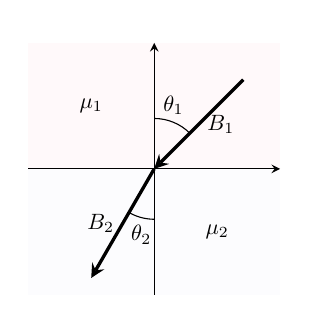
\begin{tikzpicture}[scale = 0.8, every node/.style={scale = 0.8}]
            \fill[Lavender!10] (-2,-2) rectangle (2,0);
            \fill[Pink!10] (-2,0) rectangle (2,2);
            \draw[-stealth] (-2,0) -- (2,0) node[right] {};
            \draw[-stealth] (0,-2) -- (0,2) node[above] {};
            \draw[very thick, stealth-] (0,0) -- +(45:2) node[midway,right] {$\vetor{B}_1$};
            \draw[very thick, -stealth] (0,0) -- +(-120:2) node[midway,left] {$\vetor{B}_2$};
            \draw (0,0.8) arc[start angle=90,end angle=45,radius=0.8] node[midway,above] {\(\theta_1\)};
            \draw (0,-0.8) arc[start angle=270,end angle=240,radius=0.8] node[midway, below] {\(\theta_2\)};
            \node at (-1,1) {$\mu_1$};
            \node at (1,-1) {$\mu_2$};
        \end{tikzpicture}
    \end{center}
    Assumindo que não há correntes livres na interface, utilize as condições de contorno para os campos \(\vetor{B}\) e \(\vetor{H}\) para mostrar que \(\mu_1\tan\theta_2 = \mu_2 \tan\theta_1\).
\end{exercício}
\begin{proof}[Resolução]

\end{proof}
